\chapter{Multilagen-PVD}
\label{appendix:multilayer}

\section{Porenbildung bei Unterrelaxation}

Nach der Adaptierung von Kupfer-Prozess-Parametern auf das Kupfer-Nickel-Multilagensystem konnten Multilagenabscheidungen simuliert werden, jedoch haben sich bei diesen verschiedene Defekte gebildet, die im Folgenden vorgestellt werden sollen.

Typischerweise deuten Wachstumsdefekte auf geringe Relaxationszeiten, geringe Sputterenergien oder geringe Temperaturen hin.
Das folgende System wurde bei \SI{500}{\kelvin} mit \SI{5.4}{\electronvolt} Auftreffenergie pro Teilchen für \SI{1.2}{\nano\second} relaxiert.
Die Auftreffenergie wird jedoch hauptsächlich Teil vom Thermostat abgefangen, so dass sie mit \SI{5.4}{\electronvolt} eigentlich zu niedrig liegt.

Als Resultat bilden sich Poren (Abbildung \ref{fig:multilayer_surfacefail}), die sich vergleichbar zu den Kupferkratern in Abbildung \ref{fig:coppercrater} entwickeln, sich aber erst spät wieder schließen.

\begin{figure}[h]
  \centering
  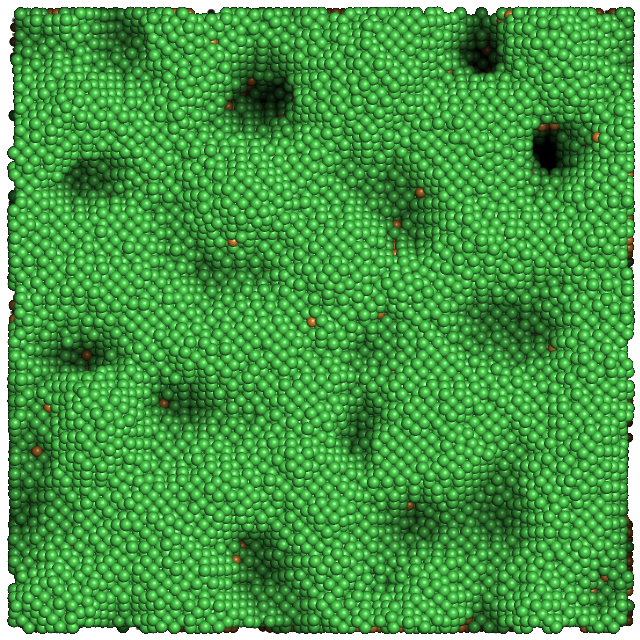
\includegraphics[height=10cm]{CuNi_surface8_noalpha}
  \caption{Draufsicht einer CuNi-Multi\-lagen\-ober\-fläche nach nur 4 Lagen (insgesamt \SI{60}{\angstrom})}
  \label{fig:multilayer_surfacefail}
\end{figure}

\clearpage
Abbildung \ref{fig:multilayer_columnfail} zeigt ein gleichartiges Resultat, das mit denselben Parametern erzeugt wurde.
Hier ist erkennbar, wie sich die gebildeten Poren wieder schließen.
Zur einfacheren Veranschaulichung wurde nur ein wenige Nanometer dünnes Profil abgebildet.

\begin{figure}[h]
  \captionsetup[subfigure]{singlelinecheck=false}
  \def\subfigwidth{7cm}
  \begin{subfigure}[t]{\subfigwidth}
    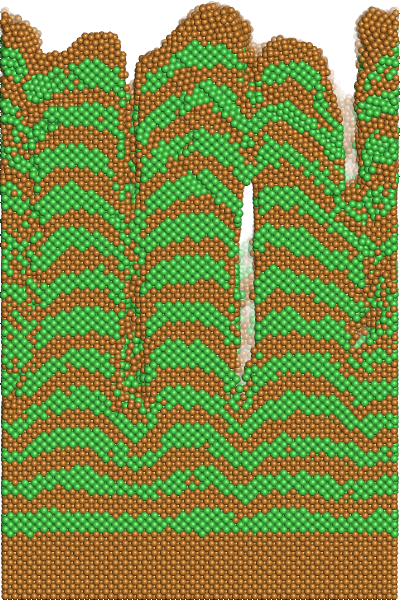
\includegraphics[width=\textwidth]{CuNi_columnfail}
    \subcaption{Dünnes Profil eines anderen Systemes nach 24 Lagen (\SI{180}{\angstrom})}
    \label{fig:multilayer_columnfail}
  \end{subfigure}
  \hfill
  \begin{subfigure}[t]{\subfigwidth}
    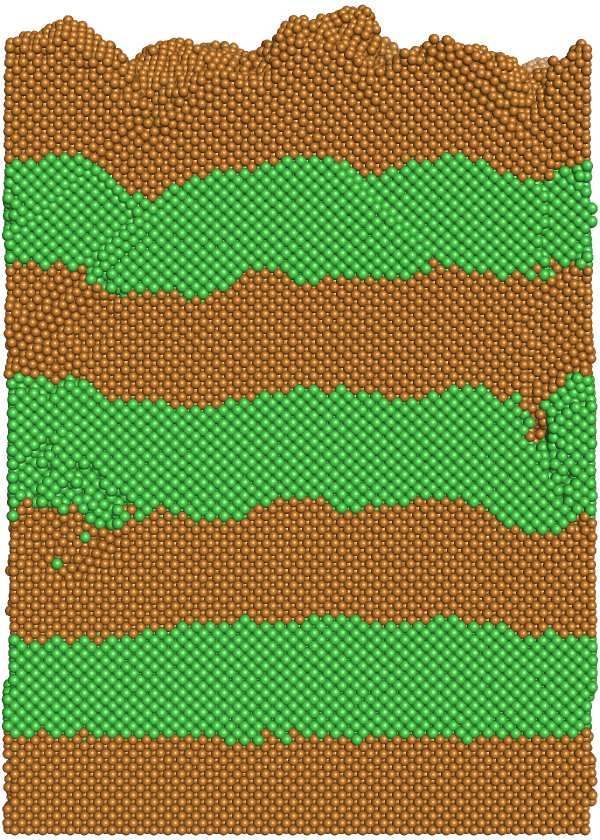
\includegraphics[width=\textwidth]{CuNi_thicklayers}
    \caption{Profil eines Systemes nach 6 Lagen je \SI{5}{\nano\meter}}
    \label{fig:multilayer_thickfail}
  \end{subfigure}
  \hfill
\end{figure}

\section{Multilagen mit einer Dicke von \SI{5}{\nano\meter}}

Ergänzend wurden auch Untersuchungen an Schichten mit Lagendicken begonnen, die sich mehr an experimentellen Werten von mehreren Nanometern orientieren.
Abbildung \ref{fig:multilayer_thickfail} stellt ein solches System dar, das aber aus Mangel an Rechenzeit für notwendige Optimierungsschritte nicht weiter untersucht wurde.
Aus diesem Grund sind auch Krater- und Porenbildungen zu beobachten, die erwartungsgemäß mit Eingabe der optimalen Werte aus Kapitel \ref{multilayer} eliminiert werden.
